\begin{abstract}
A small singular-value tail is often taken as evidence that a sequential predictor can be replaced by a small controller. We construct a single probability law on completed binary traces for which two natural readings of that inference fail. For every fixed rank budget, its Hankel operator approaches the rank-one operators in spectral norm, yet the best word-Hankel approximation at that budget has error bounded away from zero. On the same law, vanishing excess log-loss requires a proper probabilistic controller with \(L^{1-o(1)}\) states, where \(L\) is the length of one rare trace. For budgets $N=L^{\rho+o(1)}$ with $0<\rho\le1$, we determine the exact asymptotic log-loss, $M(1-\rho)\log 2$, where the exceptional trace has probability $M/L$. The proof combines a geometric waiting process and a block-enumerating trace. We also derive a test that turns one teacher-forced sequence probability into a lower bound against an entire controller class. On eight binary gate-planning instances, the test yields a \(0.7046\)-nat lower bound against one-state controllers for one constrained Qwen2.5 policy. The remaining instances delimit the power of the test.
\end{abstract}

\section{What does a small spectral tail buy?}
A planner that must act after seeing a prefix needs an update rule that remains coherent after every continuation. For a probability \(p(w)\) of a \emph{completed} action trace, the word-Hankel matrix \(H_p[u,v]=p(uv)\) encodes these continuations. Two identical concatenations have the same entry, regardless of where the split is made. An ordinary low-rank matrix approximation can break this identity; an executable weighted automaton must respect it. A probabilistic controller must also assign nonnegative probabilities and terminate with total probability one.

These requirements suggest two tests for a purported compression. First, can a linear sequential model of dimension \(k\) approximate the operator uniformly on unit input vectors? Second, can a stochastic controller with \(N\) possible internal states assign high probability to the trajectories drawn from the source? The tests quantify different errors. For the family below both tests reject the inference from a small spectral tail. They do so on the \emph{same normalized law}. The linear lower bound survives because the added trace has small operator norm. The log-loss lower bound survives because even this small probability is expensive to explain when the trace uses every length-\(m\) action block.

\paragraph{Contributions.}
We give finite inequalities for both errors, an exact state-growth exponent for vanishing log-loss, and an elementary limiting constant at rank one. The finite estimates apply before either asymptotic limit becomes informative. We use an event-level consequence to evaluate a frozen language model on fully specified planning instances, and enumerate two short-horizon laws to check the spectral diagnostic. The construction joins two separate examples in the DRAGA manuscript \cite{draga}; the contributions here are their simultaneous realization, the exact intermediate-budget tradeoff on that law, and the measured controller test. No neural training or layer removal is required by the test.

\section{Model and comparison classes}\label{sec:model}
Let \(\Sigma=\{a,b\}\), let \(\Sigma^*\) contain the empty word, and use counting measure on \(\ell^2(\Sigma^*)\). For any scalar series \(f\) with bounded word-Hankel \(H_f\), define
\[
 \delta_k(H_f)=\inf_{\rank H_g\le k}\|H_f-H_g\|_{\op},
 \qquad H_g[u,v]=g(uv).
\]
The infimum runs over bounded word-Hankels over the chosen scalar field. Finite Hankel rank is the minimal linear realization dimension \cite{carlyle,fliess}. Without the constraint on concatenations, the best rank-\(k\) error for a compact operator is \(\sigma_{k+1}\). Here \(\sigma_2\) already tends to zero.

A proper \(N\)-state controller has initial row distribution \(\alpha\), nonnegative transition matrices \(T_a,T_b\), and stop vector \(\tau=\mathbf1-(T_a+T_b)\mathbf1\ge0\). At a step it either stops or emits a symbol and changes state. Its completed-word law is \(Q(w)=\alpha T_w\tau\), with \(\sum_w Q(w)=1\). Write \(\Ckl_N(p)=\inf_Q\KL(p\Vert Q)\), taking natural logarithms. Its state includes anything that influences future actions after initialization. In particular, a time index, replay of the prefix, and access to the instance at each step would enlarge this controller interface. The source is free to use such information.

\section{One trace law with two approximation barriers}\label{sec:joint}
Fix \(k\ge1\) and \(M>0\). Let \(m\ge2\), \(K=2^m\), and \(L=mK>M\). Form \(w_m\) by concatenating the \(K\) distinct binary \(m\)-blocks in increasing lexicographic order. Set \(r=1-1/m\), \(q=1-r^2\), \(\eta=M/L\). Put mass \(h_{r,k}(a^j b^k)=(1-r)r^j\) for \(j\ge0\) and zero elsewhere. Our source is
\[
                 p_m=(1-\eta)h_{r,k}+\eta\,\mathbf{1}_{w_m}.
\]
Here \(\mathbf{1}_{w_m}\) denotes a point mass. Since \(w_m\) contains \(ba\), the two supports are disjoint. The first component describes an arbitrary wait followed by a prescribed number of actions. The second specifies an exceptional plan of length \(L\).

\begin{theorem}[Simultaneous separation]\label{th:joint}
Let \(t=(1-\eta)/(1+r)\), \(C_k=\binom{2k}{k}\), and let \(h_2\) be binary entropy in nats. Over either \(\mathbb R\) or \(\mathbb C\),
\begin{align}
 \sigma_2(H_{p_m})&\le t\sqrt q+\eta,\qquad
 \delta_k(H_{p_m})\ge t\sqrt{\frac{1+(C_k-1)q^2}{C_k}}-\eta .
 \label{eq:spec}\\
 \Ckl_N(p_m)&\ge M\log 2-\frac{M}{m}\log N-h_2(\eta),\quad N\ge1.
 \label{eq:kl}
\end{align}
Thus \(\liminf_m\delta_k(H_{p_m})\ge1/(2\sqrt{C_k})\) at fixed \(k\), while \(\sigma_2(H_{p_m})\to0\). For \(k=1\) the structured error tends to \(1/2\). For any sequence \(\epsilon_m\downarrow0\), if \(N_m^*\) is the least number of positive states with \(\Ckl_{N_m^*}(p_m)\le\epsilon_m\), then
\[
                    \lim_{m\to\infty}\frac{\log N_m^*}{\log L}=1 .
\]
\end{theorem}

\begin{theorem}[Sharp state--log-loss tradeoff]\label{th:frontier}
On the lexicographically ordered family above, suppose $N_m\ge k+2$ eventually and $\log N_m/\log L\to\rho\in[0,1]$. Then
\[
                \lim_{m\to\infty}\Ckl_{N_m}(p_m)=M(1-\rho)\log 2 .
\]
Thus a controller with $L^{1/2+o(1)}$ states pays exactly half the asymptotic log-loss of a fixed budget of at least $k+2$ states. The operator obstruction on this same law holds at fixed linear rank.
\end{theorem}

The matching controller remembers the first $\ell$ bits of the current block as a group label. Within a group, its first $\ell$ emitted bits are prescribed and its remaining bits are fair. At each block boundary it either continues the group or advances; the expected number of blocks per group equals its actual size in the witness word. Advance decisions therefore cost little total log-loss under the rare branch. This yields the finite upper bound
\[
 \Ckl_{k+2+m2^\ell}(p_m)\le M(1-\ell/m)\log2+M/m,
 \qquad 0\le\ell\le m .
\]
The ordering is essential to this upper construction. The lower bound holds in every ordering of distinct blocks.
\paragraph{Why the bounds coexist.}
The Hankel operator of a single fixed word is a partial permutation of norm one. Giving that word mass \(\eta\) changes spectral and structured distances by at most \(\eta\) relative to the scaled waiting component. For a positive controller, however, the maximum probability of the exceptional word is at most \((N/K)^K\). Each distinct \(m\)-block must draw on the same \(N\) states. Multiplication along the trace and the arithmetic--geometric mean inequality turn this shared budget into an exponentially small event probability. The supplement proves each estimate, including the matching state exponent. The family has finite mean for every \(m\), but its mean grows with \(m\). The earlier mean-bounded obstruction for log-loss alone uses another background law \cite{draga}.

\begin{figure}[t]
 \centering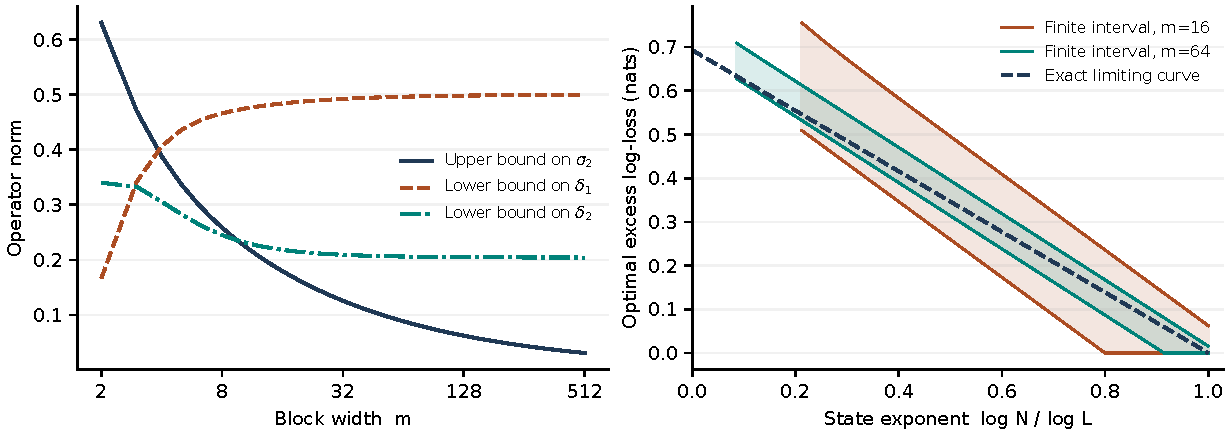
\includegraphics[width=\linewidth]{figures/joint.pdf}
 \caption{Finite certificates for the same proper law. Left: a spectral upper bound and structured lower bounds at \(k=1,2\). Right: finite upper and lower bounds and the exact asymptotic state--log-loss curve, with $k=M=1$. Curves are evaluations of inequalities, not fitted errors.}
 \label{fig:joint}
\end{figure}

\section{A test for black-box planners}\label{sec:test}
Suppose a completed plan \(w\) is the concatenation of every \(m\)-bit block once. Let \(P(w)=p\) for the policy under a fixed problem statement. For any positive \(N\)-state controller, put \(c=\min(1,(N/2^m)^{2^m})\). Observing just whether the emitted trace equals \(w\) gives
\begin{equation}
  \KL(P\Vert Q)\ge
  \begin{cases}
     p\log(p/c)+(1-p)\log((1-p)/(1-c)), &p>c,\\
     0,&p\le c.
  \end{cases} \label{eq:event}
\end{equation}
For \(N=1\) and a balanced word of length \(L\), the exact event cap is \(c=L^L/((L+1)^{L+1}2^L)\). This improves the one-state test by charging termination. A positive bound certifies a statement about every controller in the class without fitting one. Zero means that this event alone is inconclusive.

\paragraph{The gate task.}
There are \(2^m\) numbered gates. To open gate \(j\), the planner emits the \(m\) bits of \(j\), most significant first, using action A for zero and B for one. It must traverse all gates in the specified increasing or decreasing order and stop immediately. An incorrect action fails the task. The prompt supplies this rule and the endpoints. An independent verifier decodes the proposed blocks and compares their integer sequence with the required route. Success is exactly the event in \eqref{eq:event}. This is a deterministic planning task with a unique valid action trace; choosing between alternative successful plans lies outside this evaluation.

\paragraph{Checkpoint and observation.}
We evaluated the pinned four-bit ONNX export of Qwen2.5-0.5B-Instruct \cite{qwen,onnxqwen}. At every step we renormalized its logits over the same three token IDs (space-A, space-B, end-of-message). This defines the measured constrained policy. Teacher forcing scores the complete designated plan including the stop. Conditioning separately at each step differs from conditioning the original language model on the global event of valid syntax. We recorded full-vocabulary scores separately. Nontermination, if present, can be assigned to a cemetery outcome for the binary event test.

\begin{table}[ht]
\centering\small
\caption{Teacher-forced log probabilities in nats. Each target includes the final stop. The last column applies to every proper autonomous one-state controller.}\label{tab:qwen}
\begin{tabular}{rr rr rr r}\toprule
&& \multicolumn{2}{c}{Three-token policy}&\multicolumn{2}{c}{Full vocabulary}&\\
$m$ & Length & Asc. & Desc. & Asc. & Desc. & $\log c_1$\\\midrule
1 & 2 & -0.885 & -6.406 & -10.114 & -14.347 & -3.296 \\
2 & 8 & -12.932 & -11.707 & -21.962 & -20.515 & -8.685 \\
3 & 24 & -36.975 & -32.099 & -49.213 & -43.229 & -20.834 \\
4 & 64 & -72.306 & -63.446 & -88.294 & -78.497 & -49.528 \\
\bottomrule\end{tabular}
\end{table}
On the ascending two-action instance the constrained policy assigned the valid trace probability $0.4127$ (rounded). Its best one-state competitor can assign at most $1/27$. Equation~\eqref{eq:event} gives a floor of $0.7046$ nats, rounded down. The other seven one-state event tests, and all eight tests at budgets two and four, returned zero. None of the eight restricted greedy rollouts solved its instance, as determined by the first mismatch with the verified action sequence, including the stop. The full-vocabulary policy crossed none of the reported caps. A teacher-forced success probability and a greedy success indicator answer different questions.

On the two width-one prompts we also enumerated all completed traces under a three-action horizon. For ascending and descending order, the ratios $\sigma_2/\sigma_1$ were respectively 0.856 and 0.989. In both cases the antisymmetric lower bound was below $\sigma_2$. These checkpoint observations do not establish the spectral separation proved for the constructed law.


\begin{figure}[t]
\centering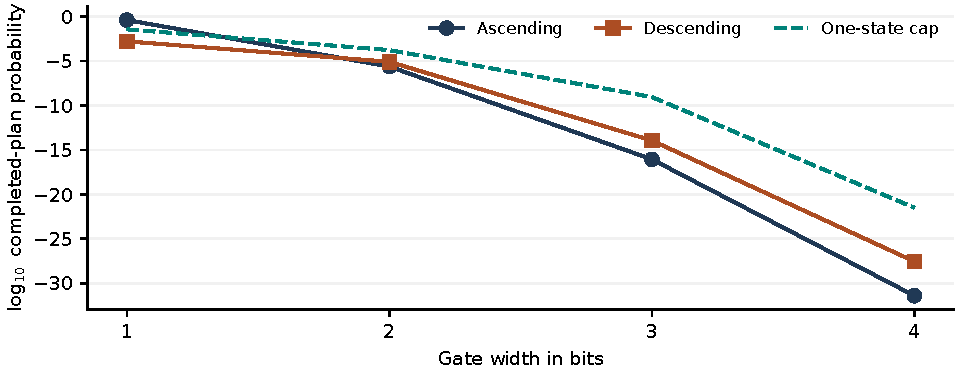
\includegraphics[width=\linewidth]{figures/planner.pdf}
\caption{Log probability of the verifier-accepted action trace under the constrained checkpoint, by gate width and order. The dashed line is the analytic one-state cap; a point above that line certifies positive excess log-loss. Lines between discrete widths guide the eye.}
\label{fig:planner}
\end{figure}

\section{Related work and scope}\label{sec:limits}
Classical realization theory identifies finite rank with linear state dimension \cite{carlyle,fliess}. Singular value automata support spectral truncation under specific guarantees \cite{sva}. Exact spectral-norm approximate minimization is established for one-letter weighted automata \cite{unary}; the multiletter work of Lacroce et al.\ develops a noncommutative formulation \cite{multi}. Our comparison uses the ordinary word-Hankel on counting measure, its concatenation identities and uniform operator norm. Predictive representations use tests of future observations \cite{psr}. Black-box extraction can learn automata from numerical sequence queries \cite{ayache}. Our certificate bounds the error of the entire comparison class. Classical finite-state coding lower bounds \cite{lz} and approximate HMM realization under divergence rate \cite{hmm} supply related viewpoints. We consider the total log-loss on completed finite traces.

The fixed-\(k\) operator example approaches the boundary of stability. The bounds do not quantify approximation on a uniformly stable family, on natural-language text, or for an unrestricted neural architecture with real-valued recurrent state. The KL certificate concerns a declared autonomous finite controller; it gives neither a layer count nor a hardware-byte lower bound for a Transformer or Gated DeltaNet. One quantized checkpoint and eight designed tasks support an audit of the certificate. Broader claims about planning competence would require other tasks, alternative successful trajectories, and more model families.
